\section{Multi-commodity flow and SR}

%The only difference between the two is that the MCFP allows for several paths to be used of the same demand.

\vspace{0.5cm}


In this section we propose a new TE solution that consists of leveraging our minimal segmentation algorithm
to segment the optimal solution of the MCFP. The MCPF can be solved in polynomial time since we can
express is as a linear problem \todo{ref LP in P}. One possible LP formulation is the following.


Given a solution matrix $x$ to \mcflp~we can easily construct a set of paths for each demand $d = (s, t, \nu) \in \mathcal{D}$.
To do so, we perform a sequence of breadth-first searches (BFS) from $s$ following only edges $e$ such that $x_{ed} > 0$. Each time we reach $t$, we 
trace back the path $p$ and reduce the value of $x_{ed}$ by the $\min_{e \in E(p)} x_{ed}$. We continue to do this until one of the searches
fails to reach $t$. At this point we finished computing a set of paths for demand $d$. Repeating the process for each demand will yield a set of 
paths over which we can route the demands without exceeding the capacity of any edge by a factor greater than $\lambda$. 

Figure \ref{fig:flow-path} illustrates this process on a small example. The graph represents the values of $x_{ed}$ for a specific demand $d$. Each edge
if labeled with the value of $x_{ed}$ (for clarity, we ommit edge with value $0$ since they are ignored anyway by the DFS). Then the blue arrows show possible
BFS paths. After each path is found, the value of the edges is reduced until no more paths exist. In this case we get three paths: 
$((\node{a}, \node{b}), (\node{b}, \node{d}))$, $((\node{a}, \node{c}), (\node{c}, \node{d}))$ and $((\node{a}, \node{b}), (\node{b}, \node{c}), (\node{c}, \node{d}))$.

\begin{figure}
\begin{center}
\begin{tabular}{c c c}
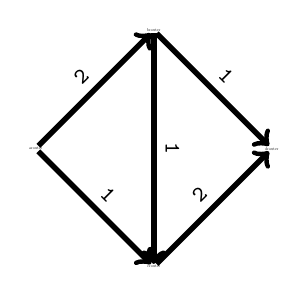
\begin{tikzpicture}
\node[scale=0.15] (a) at (0, 0) {\router{a}{router}};
\node[scale=0.15] (b) at (1.5, 1.5) {\router{b}{router}};
\node[scale=0.15] (c) at (1.5, -1.5) {\router{c}{router}};
\node[scale=0.15] (d) at (3, 0) {\router{d}{router}};
\draw[line width=2] (a) edge[above, sloped, ->] node[black,font=\bfseries] {\footnotesize \texttt{2}} (b);
%\draw[line width=2] (b) edge[below, sloped, bend left = 10, ->] node[black,font=\bfseries] {\tiny \texttt{0}} (a);

\draw[line width=2] (a) edge[above, sloped, ->] node[black,font=\bfseries] {\footnotesize \texttt{1}} (c);
%\draw[line width=2] (c) edge[below, sloped, bend left = 10, ->] node[black,font=\bfseries] {\tiny \texttt{0}} (a);

\draw[line width=2] (b) edge[above, sloped, ->] node[black,font=\bfseries] {\footnotesize \texttt{1}} (d);
%\draw[line width=2] (d) edge[below, sloped, bend left = 10, ->] node[black,font=\bfseries] {\tiny \texttt{0}} (b);

\draw[line width=2] (c) edge[above, sloped, ->] node[black,font=\bfseries] {\footnotesize \texttt{2}} (d);
%\draw[line width=2] (d) edge[below, sloped, bend left = 10, ->] node[black,font=\bfseries] {\tiny \texttt{0}} (c);

\draw[line width=2] (b) edge[above, sloped, ->] node[black,font=\bfseries] {\footnotesize \texttt{1}} (c);
%\draw[line width=2] (c) edge[below, sloped, bend left = 10, ->] node[black,font=\bfseries] {\tiny \texttt{0}} (b);
\end{tikzpicture}

&

\begin{tikzpicture}
\node[scale=0.15] (a) at (0, 0) {\router{a}{router}};
\node[scale=0.15] (b) at (1.5, 1.5) {\router{b}{router}};
\node[scale=0.15] (c) at (1.5, -1.5) {\router{c}{router}};
\node[scale=0.15] (d) at (3, 0) {\router{d}{router}};
\draw[line width=2] (a) edge[above, sloped, ->] node[black,font=\bfseries] {\footnotesize \texttt{2}} (b);
%\draw[line width=2] (b) edge[below, sloped, bend left = 10, ->] node[black,font=\bfseries] {\tiny \texttt{0}} (a);

\draw[line width=2] (a) edge[above, sloped, ->] node[black,font=\bfseries] {\footnotesize \texttt{1}} (c);
%\draw[line width=2] (c) edge[below, sloped, bend left = 10, ->] node[black,font=\bfseries] {\tiny \texttt{0}} (a);

\draw[line width=2] (b) edge[above, sloped, ->] node[black,font=\bfseries] {\footnotesize \texttt{1}} (d);
%\draw[line width=2] (d) edge[below, sloped, bend left = 10, ->] node[black,font=\bfseries] {\tiny \texttt{0}} (b);

\draw[line width=2] (c) edge[above, sloped, ->] node[black,font=\bfseries] {\footnotesize \texttt{2}} (d);
%\draw[line width=2] (d) edge[below, sloped, bend left = 10, ->] node[black,font=\bfseries] {\tiny \texttt{0}} (c);

\draw[line width=2] (b) edge[above, sloped, ->] node[black,font=\bfseries] {\footnotesize \texttt{1}} (c);
%\draw[line width=2] (c) edge[below, sloped, bend left = 10, ->] node[black,font=\bfseries] {\tiny \texttt{0}} (b);


\draw[cyan, line width=2, ->] plot [smooth] coordinates { ($(a)+(0,0.5)$) ($(b)+(0,0.75)$) ($(d)+(0,0.5)$) };

\end{tikzpicture}

&

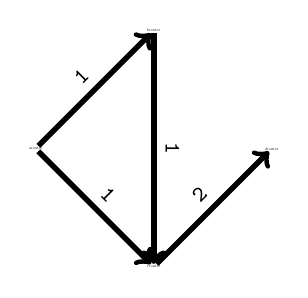
\begin{tikzpicture}
\node[scale=0.15] (a) at (0, 0) {\router{a}{router}};
\node[scale=0.15] (b) at (1.5, 1.5) {\router{b}{router}};
\node[scale=0.15] (c) at (1.5, -1.5) {\router{c}{router}};
\node[scale=0.15] (d) at (3, 0) {\router{d}{router}};
\draw[line width=2] (a) edge[above, sloped, ->] node[black,font=\bfseries] {\footnotesize \texttt{1}} (b);
%\draw[line width=2] (b) edge[below, sloped, bend left = 10, ->] node[black,font=\bfseries] {\tiny \texttt{0}} (a);

\draw[line width=2] (a) edge[above, sloped, ->] node[black,font=\bfseries] {\footnotesize \texttt{1}} (c);
%\draw[line width=2] (c) edge[below, sloped, bend left = 10, ->] node[black,font=\bfseries] {\tiny \texttt{0}} (a);

%\draw[line width=2] (b) edge[above, sloped, ->] node[black,font=\bfseries] {\footnotesize \texttt{1}} (d);
%\draw[line width=2] (d) edge[below, sloped, bend left = 10, ->] node[black,font=\bfseries] {\tiny \texttt{0}} (b);

\draw[line width=2] (c) edge[above, sloped, ->] node[black,font=\bfseries] {\footnotesize \texttt{2}} (d);
%\draw[line width=2] (d) edge[below, sloped, bend left = 10, ->] node[black,font=\bfseries] {\tiny \texttt{0}} (c);

\draw[line width=2] (b) edge[above, sloped, ->] node[black,font=\bfseries] {\footnotesize \texttt{1}} (c);
%\draw[line width=2] (c) edge[below, sloped, bend left = 10, ->] node[black,font=\bfseries] {\tiny \texttt{0}} (b);

\end{tikzpicture}

\\

(1) Solution graph

&

(2) First BFS

&

(3) Graph after reweight

\\[0.5cm]

\begin{tikzpicture}
\node[scale=0.15] (a) at (0, 0) {\router{a}{router}};
\node[scale=0.15] (b) at (1.5, 1.5) {\router{b}{router}};
\node[scale=0.15] (c) at (1.5, -1.5) {\router{c}{router}};
\node[scale=0.15] (d) at (3, 0) {\router{d}{router}};
\draw[line width=2] (a) edge[above, sloped, ->] node[black,font=\bfseries] {\footnotesize \texttt{1}} (b);
%\draw[line width=2] (b) edge[below, sloped, bend left = 10, ->] node[black,font=\bfseries] {\tiny \texttt{0}} (a);

\draw[line width=2] (a) edge[above, sloped, ->] node[black,font=\bfseries] {\footnotesize \texttt{1}} (c);
%\draw[line width=2] (c) edge[below, sloped, bend left = 10, ->] node[black,font=\bfseries] {\tiny \texttt{0}} (a);

%\draw[line width=2] (b) edge[above, sloped, ->] node[black,font=\bfseries] {\footnotesize \texttt{1}} (d);
%\draw[line width=2] (d) edge[below, sloped, bend left = 10, ->] node[black,font=\bfseries] {\tiny \texttt{0}} (b);

\draw[line width=2] (c) edge[above, sloped, ->] node[black,font=\bfseries] {\footnotesize \texttt{2}} (d);
%\draw[line width=2] (d) edge[below, sloped, bend left = 10, ->] node[black,font=\bfseries] {\tiny \texttt{0}} (c);

\draw[line width=2] (b) edge[above, sloped, ->] node[black,font=\bfseries] {\footnotesize \texttt{1}} (c);
%\draw[line width=2] (c) edge[below, sloped, bend left = 10, ->] node[black,font=\bfseries] {\tiny \texttt{0}} (b);

\draw[cyan, line width=2, ->] plot [smooth] coordinates { ($(a)+(0,-0.5)$) ($(c)+(0,-0.75)$) ($(d)+(0,-0.5)$) };


\end{tikzpicture}

&

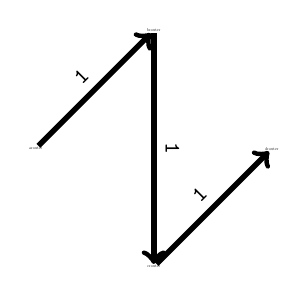
\begin{tikzpicture}
\node[scale=0.15] (a) at (0, 0) {\router{a}{router}};
\node[scale=0.15] (b) at (1.5, 1.5) {\router{b}{router}};
\node[scale=0.15] (c) at (1.5, -1.5) {\router{c}{router}};
\node[scale=0.15] (d) at (3, 0) {\router{d}{router}};
\draw[line width=2] (a) edge[above, sloped, ->] node[black,font=\bfseries] {\footnotesize \texttt{1}} (b);
%\draw[line width=2] (b) edge[below, sloped, bend left = 10, ->] node[black,font=\bfseries] {\tiny \texttt{0}} (a);

%\draw[line width=2] (a) edge[above, sloped, ->] node[black,font=\bfseries] {\footnotesize \texttt{1}} (c);
%\draw[line width=2] (c) edge[below, sloped, bend left = 10, ->] node[black,font=\bfseries] {\tiny \texttt{0}} (a);

%\draw[line width=2] (b) edge[above, sloped, ->] node[black,font=\bfseries] {\footnotesize \texttt{1}} (d);
%\draw[line width=2] (d) edge[below, sloped, bend left = 10, ->] node[black,font=\bfseries] {\tiny \texttt{0}} (b);

\draw[line width=2] (c) edge[above, sloped, ->] node[black,font=\bfseries] {\footnotesize \texttt{1}} (d);
%\draw[line width=2] (d) edge[below, sloped, bend left = 10, ->] node[black,font=\bfseries] {\tiny \texttt{0}} (c);

\draw[line width=2] (b) edge[above, sloped, ->] node[black,font=\bfseries] {\footnotesize \texttt{1}} (c);
%\draw[line width=2] (c) edge[below, sloped, bend left = 10, ->] node[black,font=\bfseries] {\tiny \texttt{0}} (b);

%\draw[cyan, line width=2, ->] plot [smooth] coordinates { ($(a)+(0,-0.5)$) ($(c)+(0,-0.75)$) ($(d)+(0,-0.5)$) };


\end{tikzpicture}

&

\begin{tikzpicture}
\node[scale=0.15] (a) at (0, 0) {\router{a}{router}};
\node[scale=0.15] (b) at (1.5, 1.5) {\router{b}{router}};
\node[scale=0.15] (c) at (1.5, -1.5) {\router{c}{router}};
\node[scale=0.15] (d) at (3, 0) {\router{d}{router}};
\draw[line width=2] (a) edge[above, sloped, ->] node[black,font=\bfseries] {\footnotesize \texttt{1}} (b);
%\draw[line width=2] (b) edge[below, sloped, bend left = 10, ->] node[black,font=\bfseries] {\tiny \texttt{0}} (a);

%\draw[line width=2] (a) edge[above, sloped, ->] node[black,font=\bfseries] {\footnotesize \texttt{1}} (c);
%\draw[line width=2] (c) edge[below, sloped, bend left = 10, ->] node[black,font=\bfseries] {\tiny \texttt{0}} (a);

%\draw[line width=2] (b) edge[above, sloped, ->] node[black,font=\bfseries] {\footnotesize \texttt{1}} (d);
%\draw[line width=2] (d) edge[below, sloped, bend left = 10, ->] node[black,font=\bfseries] {\tiny \texttt{0}} (b);

\draw[line width=2] (c) edge[above, sloped, ->] node[black,font=\bfseries] {\footnotesize \texttt{1}} (d);
%\draw[line width=2] (d) edge[below, sloped, bend left = 10, ->] node[black,font=\bfseries] {\tiny \texttt{0}} (c);

\draw[line width=2] (b) edge[above, sloped, ->] node[black,font=\bfseries] {\footnotesize \texttt{1}} (c);
%\draw[line width=2] (c) edge[below, sloped, bend left = 10, ->] node[black,font=\bfseries] {\tiny \texttt{0}} (b);

\draw[cyan, line width=2, ->] plot [smooth] coordinates { ($(a)+(0,0.5)$) ($(b)+(0,0.75)$) ($(b)+(0.75,0)$)  ($(b)+(0,-1)$) ($(c)+(-0.75,0)$) ($(c)+(0,-0.75)$) ($(d)+(0,-0.75)$)};

\end{tikzpicture}


\\

(4) Second BFS

&

(5) Graph after reweight

&

(6) Third BFS

\end{tabular}
\end{center}
\label{fig:flow-path}
\caption{Converting the flow to a path set.}
\end{figure}

Using this procedure, we can easily transform a solution of \mcflp~in a solution 
$\mathcal{P}_1, \ldots, \mathcal{P}_r$ of Problem \ref{prob:tep-mul}. To implement such a solution 
on a network with segment routing we can simply use our minimum segmentation algorithm.
Algorithm \ref{algo:mcf-seg} provides a formal descrition on how we can combine \mcflp~with
the minimum segmentation algorithm to provide an optimal solution to Problem \ref{prob:tep-mul}
implementable with segment routing.

\begin{algorithm}[t]
\small
\caption{$\textsf{sr-MCF}\left( G, \mathcal{D} \right)$}
\begin{algorithmic}[1]
\STATE $x \gets \textsf{LP-SOLVE}(\textsf{MCF-LP}(G, \mathcal{D}))$ \label{line:srmcf_lp}
\STATE $\mathcal{P} \gets \emptyset$
\FOR{$d \in \mathcal{D}$}
  \STATE $G_d \gets (V, \{ e \in E(G) \mid x_{ed} > 0 \})$ \label{line:srmcf_buildg}
  \STATE $p \gets \textsf{BFS}(G_d, src(d), dst(d))$ \label{line:srmcf_p1}
  \WHILE{$p \neq \bot$} \label{line:srmcf_while}
    \STATE $\Delta \gets \min_{e \in E(p)} x_{ed}$ \label{line:srmcf_delta}
    \STATE $\mathcal{P} \gets \mathcal{P} \cup \{ (p, \Delta) \}$ \label{line:srmcf_add}
    \FOR{$e \in E(p)$} \label{line:srmcf_for}
      \STATE $x_{ed} \gets x_{ed} - \Delta$ \label{line:srmcf_update}
    \ENDFOR
    \STATE $G_d \gets (V, \{ e \in E(G) \mid x_{ed} > 0 \})$ \label{line:srmcf_buildgw}
    \STATE $p \gets \textsf{BFS}(G_d, src(d), dst(d))$ \label{line:srmcf_pw}
  \ENDWHILE
\ENDFOR
\RETURN $\{ (\textsf{min-seg}(G, p), \Delta) \mid (p, \Delta) \in \mathcal{P} \}$
\end{algorithmic}
\label{algo:mcf-seg}
\end{algorithm}

\begin{proposition}
Algorithm \ref{algo:mcf-seg} runs in polynomial time.
\end{proposition}

\begin{proof}
We know that linear problems can be solved in polynomial time \todo{ref}. Therefore compute $x$ can be done in polynomial time on line \ref{line:srmcf_lp}.
It remains to show that our path building process take polynomial time. Let $d \in \mathcal{D}$. Building the graph $G_d$ on line \ref{line:srmcf_buildg} takes
$O(|E(G)| \cdot |\mathcal{D}|)$ and each \textsf{BFS} call takes $O(|G|)$. In body of the while loop, that is, lines \ref{line:srmcf_delta}
to \ref{line:srmcf_pw}, the most costly line is line \ref{line:srmcf_pw} which takes $O(|V(G)| \cdot |E(G)|)$. Therefore we only need to prove that the number 
of iterations of the while loop is polynomial. Since $\Delta = \min_{e \in E(p)} x_{ed}$, at each iteration, at least one edge is removed from $G_d$ at
line \ref{line:srmcf_buildgw}. This means that the number of iterations of the while loop is at most $|E(G)|$ giving a total runtime of
$O(LP + |\mathcal{D}| \cdot (|G| + |E(G)| \cdot |G|)) = O(LP + |\mathcal{D}| \cdot |G| \cdot |E(G)|)$.
\end{proof}

\todo{OBO: what are the practical limitations of using several paths per demand? Should we write a few pages about this? because this problem really is more easy to solve}

As with any solution that consists of solving a problem on the original network $G$ and only after segments the paths,
this solutions has the huge drawback that it fails to provide control on the number of segments needed to implement the 
solution. We executed this algorithm on our data set and analysed the number of segments necessary in these solutions.

\todo{show plots and discuss}